% \documentclass{standalone}
\documentclass[tikz,convert={outfile=\jobname.svg}]{standalone}
\usepackage{tikz}
\begin{document}
\tikzset{
every picture/.style={
  execute at end picture={
    \path (current bounding box.south west) +(-1,-1) (current bounding box.north east) +(1,1);
    }
  }
}
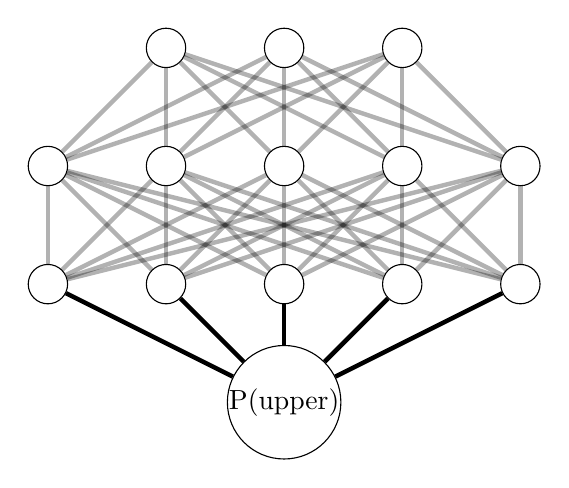
\begin{tikzpicture}[
    roundnode/.style={circle, draw=black, minimum size=5mm, inner sep=0pt},
    squarednode/.style={draw=black, minimum size=5mm, inner sep=2pt},
    ]

% First layer
\node[roundnode] (n1) at (0,1.5) {};
\node[roundnode] (n2) at (1.5,1.5) {};
\node[roundnode] (n3) at (3,1.5) {};
\node[roundnode] (n4) at (4.5,1.5) {};
\node[roundnode] (n5) at (6,1.5) {};

% Second layer
\node[roundnode] (n6) at (0,3) {};
\node[roundnode] (n7) at (1.5,3) {};
\node[roundnode] (n8) at (3,3) {};
\node[roundnode] (n9) at (4.5,3) {};
\node[roundnode] (n10) at (6,3) {};

% Third layer
\node[roundnode] (n11) at (1.5,4.5) {};
\node[roundnode] (n12) at (3,4.5) {};
\node[roundnode] (n13) at (4.5,4.5) {};

% Last layer
\node[roundnode] (n14) at (3,0) {P(upper)};
% \node[draw, shape=ellipse, minimum width=3cm, minimum height=1.5cm] (n14) at (3,0) {P(upper)};
% \draw (3,0) ellipse (1.5cm and 0.7cm);

% Edges between layers
\foreach \i in {1,2,3,4,5} {
    \foreach \j in {6,7,8,9,10} {
        \draw[ultra thick, opacity=0.3] (n\i) -- (n\j);
    }
}

\foreach \i in {6,7,8,9,10} {
    \foreach \j in {11,12,13} {
        \draw[ultra thick, opacity=0.3] (n\i) -- (n\j);
    }
}

\foreach \i in {1,2,3,4,5} {
    \draw[ultra thick] (n\i) -- (n14);
}

\end{tikzpicture}

\end{document}
